\chapter{Estimation du seuil optimale par des indicateurs sonores}\label{annexe:optThreshold}

Dans la partie \ref{}, les seuils optimaux par ambiance sonores ont été défini en considérant la NMF IS optimale avec $\beta$ = 2, $K$ = 300 et $w_t$ = 1 s. Les seuils optimaux et l'erreur correspondante par ambiance sont résumées dans le Tableau \ref{tab:erreur_optimiseAnn}.
Ces seuils pouvaient être considérés notamment dans les réseaux de capteurs fixes où l'ESU peut être défini au préalable. Toutefois, leur prise en compte a un impact relativement faible sur les erreurs. 

Cependant, une piste a été étudié en vue de, non plus définir un seuil fixe selon l'ambiance sonore, mais de définir un seuil adaptatif basé sur des indicateurs physiques corrélés avec l'évolution des seuils optimaux. Cette adaptation permettrait, pour les réseaux de capteurs fixes, de s'adapter à des ESU qui peuvent évolués aux alentours des microphones selon la période dans l'année ou dans la journée.

\begin{table}[h]
\centering
\caption{Erreurs $MAE_{60}$ minimales selon le seuil optimal $t_{h,opt}$ par ambiance sonore.}
\label{tab:erreur_optimiseAnn}
\resizebox{\textwidth}{!}{%
\begin{tabular}{L{4cm}C{2.5cm}C{2.5cm}C{2.5cm}C{2.5cm}C{2.5cm}}
\toprule
 & Parc & Rue Calme & Rue Bruyante & Rue très bruyante & $MAE_{60}$ \\
\midrule
seuil fixe $t_h$ & 0,35 & 0,35 & 0,35 & 0,35 & - \\
erreur $MAE_{60}$ & 2,13 ($\pm$ 3,84) & 1,62 ($\pm$ 1,85) & 0,57 ($\pm$ 0,54) &  0,32 ($\pm$ 0,20) & 1,16 ($\pm$ 0,86) \\
\midrule
seuil optimal $t_{h,opt.}$ & 0,38 & 0,35 & 0,33 & 0,31 & - \\
erreur $MAE_{60}$ & 2,03 ($\pm$ 3,47) & 1,62 ($\pm$ 1,85) & 0,56 ($\pm$ 0,67) & 0,28 ($\pm$ 0,31) & 1,12 ($\pm$ 0,83)\\
\bottomrule
\end{tabular}}
\end{table}


Des outils de classification pour les environnements sonores existent déjà dans la littérature basé sur des indicateurs simples (\cite{can_describing_2015}, \cite{rychtarikova2013soundscape}) ou sur des outils plus complexe comme dans \cite{salamon2015unsupervised}.
Dans le cadre de ces travaux, il est nécessaire que ces indicateurs soient simples en vue de considérer cette méthode sur l'ensemble des types de mesures possible (fixes, mobiles, participatives sur smartphones) dont les puissances de calculs sont limités. Ainsi, nous considérons une approche simple basée sur l'estimation d'indicateurs de niveaux sonores.
Le principe consiste alors à déterminer un indicateur dont son évolution selon les ambiance sonores est corrélé à celles des seuil optimaux. Ainsi à partir de cet estimation, il sera possible de définir un seuil optimal adapté à l'ESU de la mesure.
Plusieurs indicateurs sont considérés comme des niveaux sonores par bandes de tiers d'octaves ($L_{500}$, $L_{1000}$, $L_{2000}$, $L_{5000}$) ainsi que des niveaux sonores fractiles ($L_{10}$, $L_{50}$, $L_{90}$). Ces derniers exprime les niveaux sonores dépassés pendant une période définie. Ainsi $L_{10}$ exprime le niveau sonore dépassé 10 $\%$ du temps, cela résume les hauts niveaux sonores, à l'inverse l'indice $L_{90}$ traduit le niveau sonore dépassé 90 $\%$ du temps et exprime donc l'équivalent du bruit de fond sonore d'une scène.

Toutefois, cette approche se heurte à la calibration des scènes sonores. En effet, les scènes sonores sont composées sur un modèle relatif : les classes de sons présentes et leur émergences sont choisies en fonction des autres sources sonores et du bruit de fond sonore. L'ambiance sonore souhaité, est donc obtenue en fonction des classes de sons présente et leur émergence dans la scène. La connaissance du niveau sonore globale de la scène n'est alors pas nécessaire en vu d'estimer la contribution sonore du trafic routier.
Ainsi, pour pouvoir comparer les niveaux sonores les scènes sonores simulées en fonction des ambiances sonores, il est nécessaire que celle-ci soient calibrées par rapport aux niveaux sonores des enregistrements audio dont elles s'inspirent. Malheureusement, les enregistrements audio \textit{GRAFIC} récupérés n'ont pas été accompagnés d'un fichier de calibration. Il est donc impossible d'estimer correctement des niveaux sonores globaux absolus comme le niveau sonore global pondéré $A$ par exemple. Une approximation avait été réalisée dans le Tableau \ref{tab:obsScene} à partir des informations données dans la Figure \ref{fig:parcoursGRAFIC}, mais celle-ci n'est pas suffisante ici.

Considérant que les scènes du corpus \textit{SOUR} sont représentatives d'enregistrements sonores urbains, si ces niveaux absolus des indicateurs de niveaux sonores ne sont pas correctes par défaut de calibration, leurs rapports entre eux l'est tout de même.
Ainsi la différence entre les niveaux par bandes de tiers d'octaves et entre les niveaux fractiles sont calculées : 

\begin{subequations}\label{eq:delta_L}
\begin{align}
\Delta_{L_{500}-L_{1000}} &= L_{500}-L_{1000}, \\
\Delta_{L_{500}-L_{2000}} &= L_{500}-L_{2000}, \\
\Delta_{L_{500}-L_{5000}} &= L_{500}-L_{5000}, \\
\Delta_{L_{1000}-L_{2000}} &= L_{1000}-L_{2000}, \\
\Delta_{L_{1000}-L_{5000}} &= L_{1000}-L_{5000}, \\
\Delta_{L_{2000}-L_{5000}} &= L_{500}-L_{5000}, \\
\Delta_{L_{10}-L_{50}} &= L_{10}-L_{50}, \\
\Delta_{L_{10}-L_{90}} &= L_{10}-L_{90}, \\
\Delta_{L_{50}-L_{90}} &= L_{50}-L_{90}.
\end{align}
\end{subequations}

\begin{figure}[h]
\centering
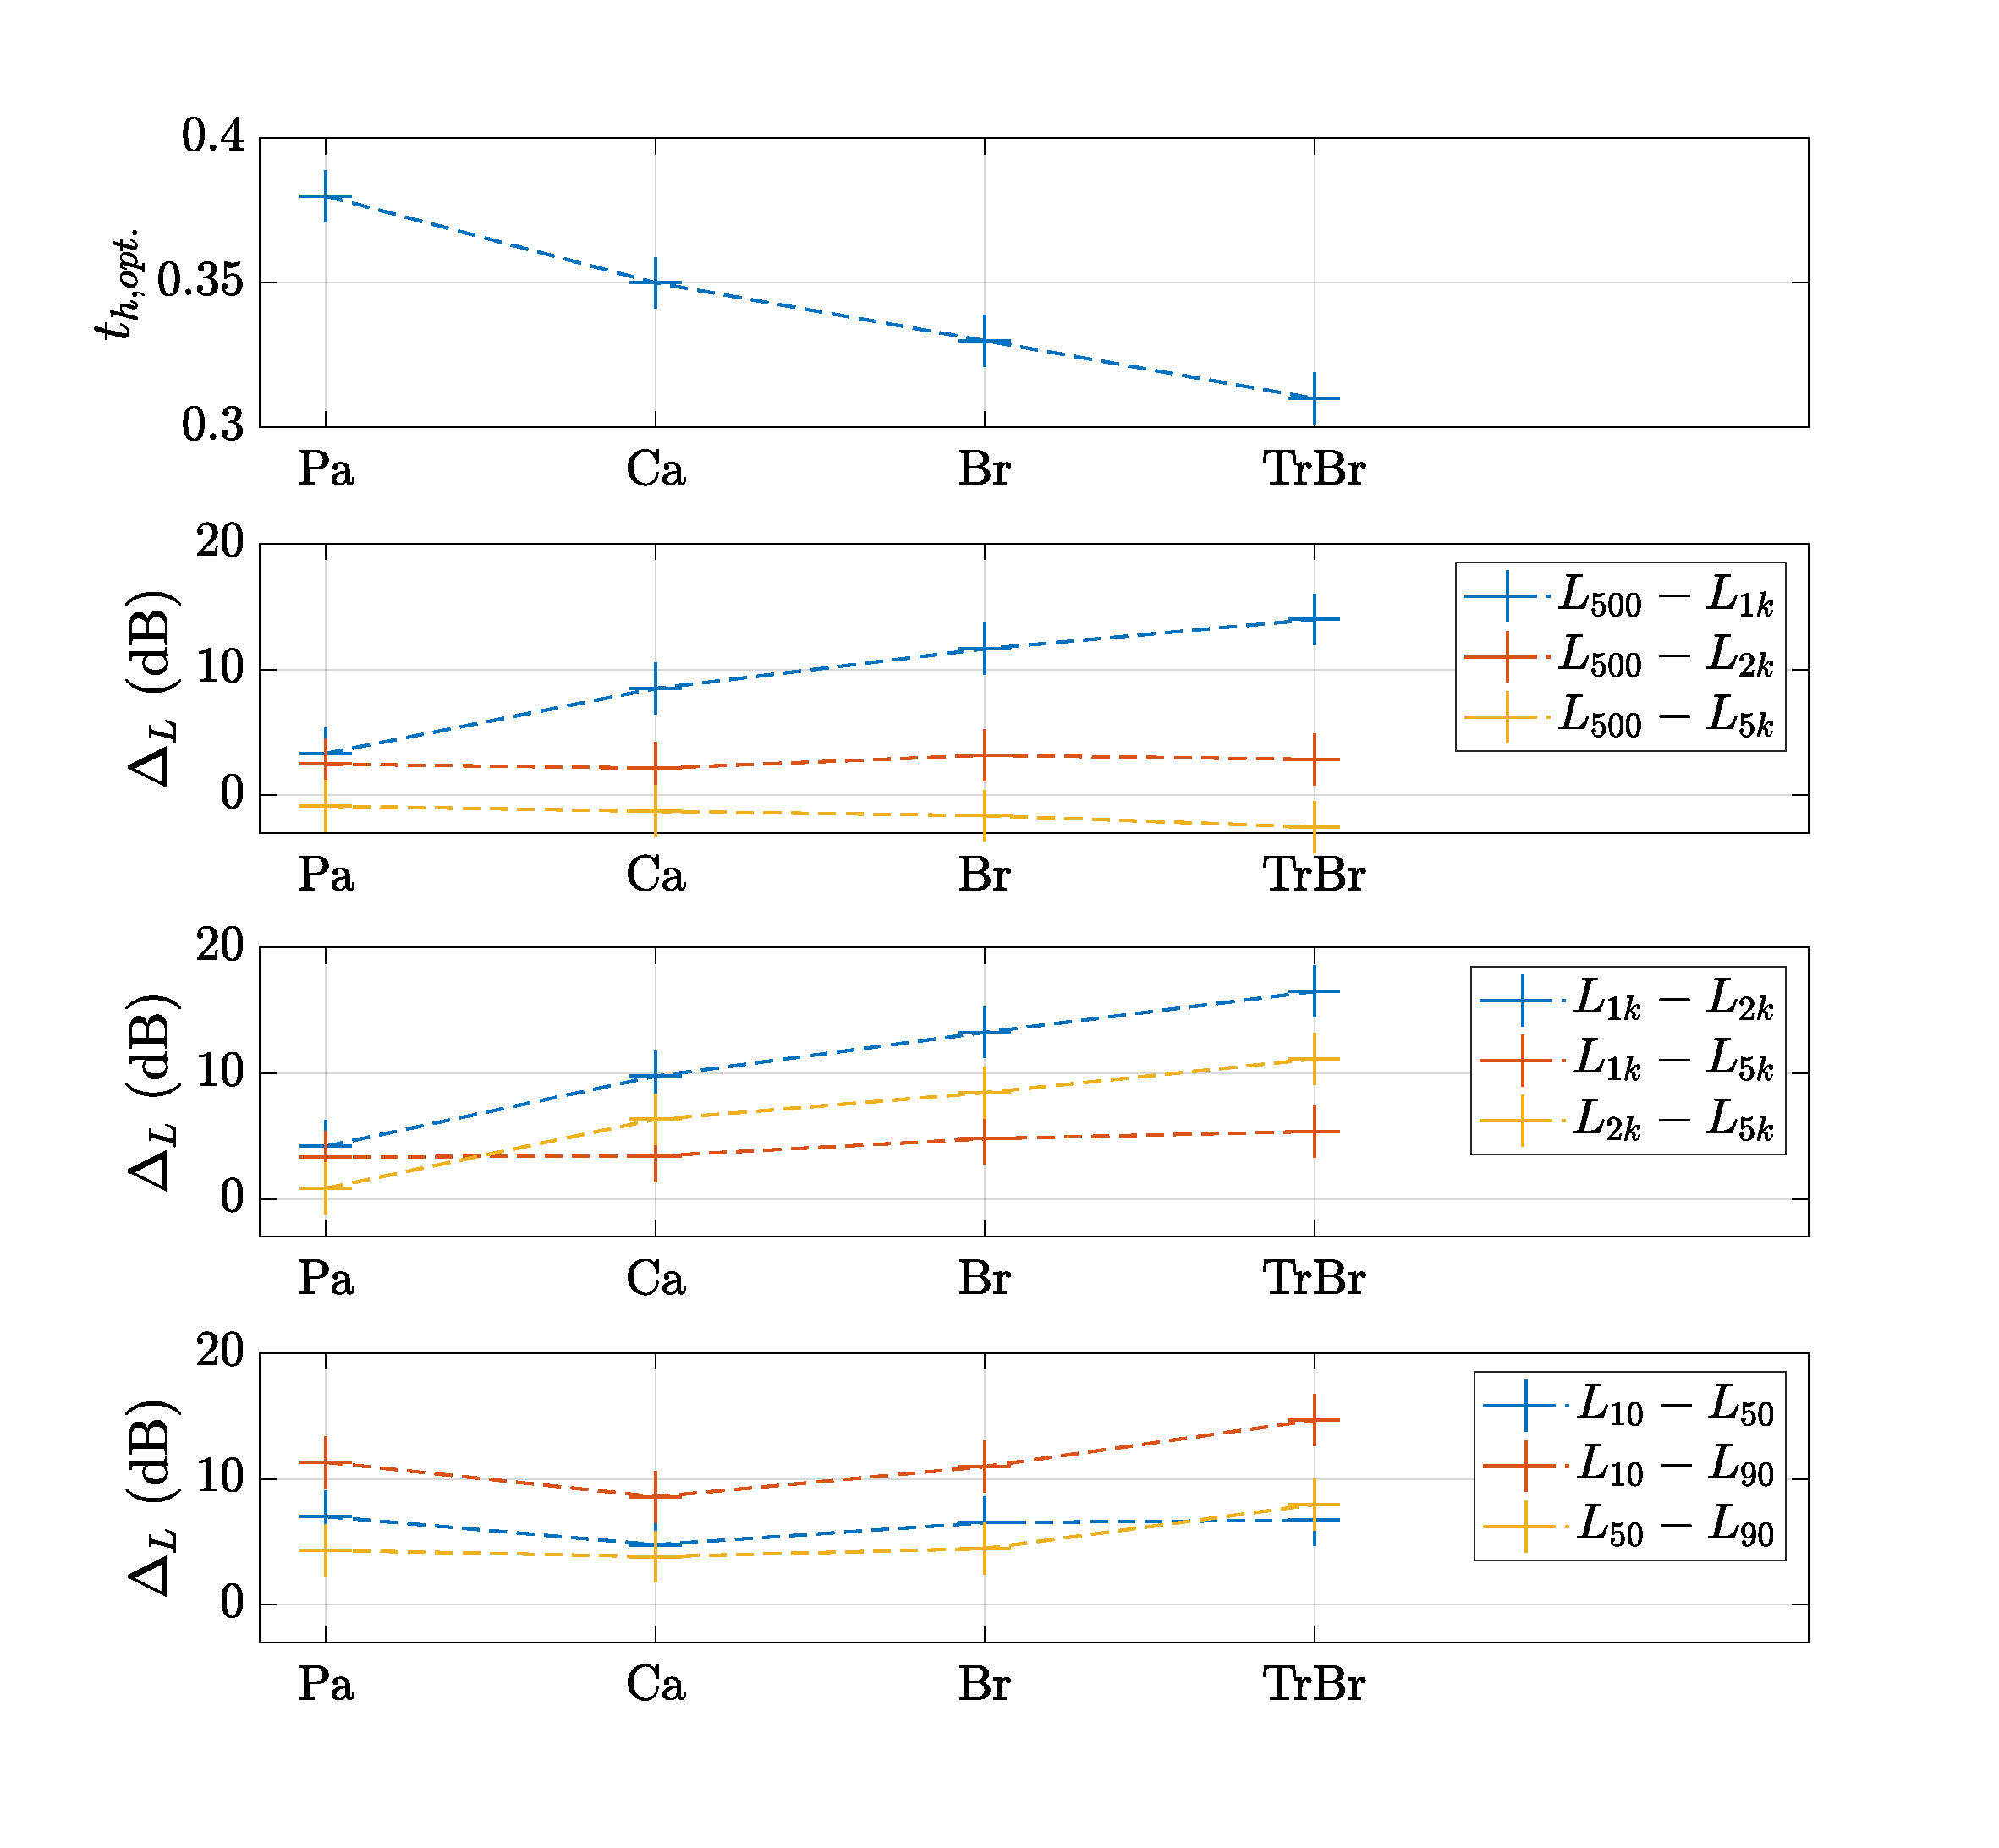
\includegraphics[width=0.9\linewidth]{./figures/resultats/deltaL_opt.pdf}
\caption{Évolution des seuils optimaux et des indicateurs $\Delta_L$ selon les ambiances.}
\label{fig:delta_L}
\end{figure}


La Figure \ref{fig:delta_L} résume les évolutions du seuil optimal et des indicateurs $\Delta_{L_x-L_y}$ par ambiance sonore. \`A partir de ces valeurs, la corrélation entre l'évolution du seuil optimale par ambiance sonore et celle des indicateurs est alors calculée pour déterminer quelle indicateur évolue de la même façon que les seuils optimaux. Les valeurs absolues des corrélations sont résumées dans le Tableau \ref{fig:correlation}.

\begin{figure}[h]
\centering
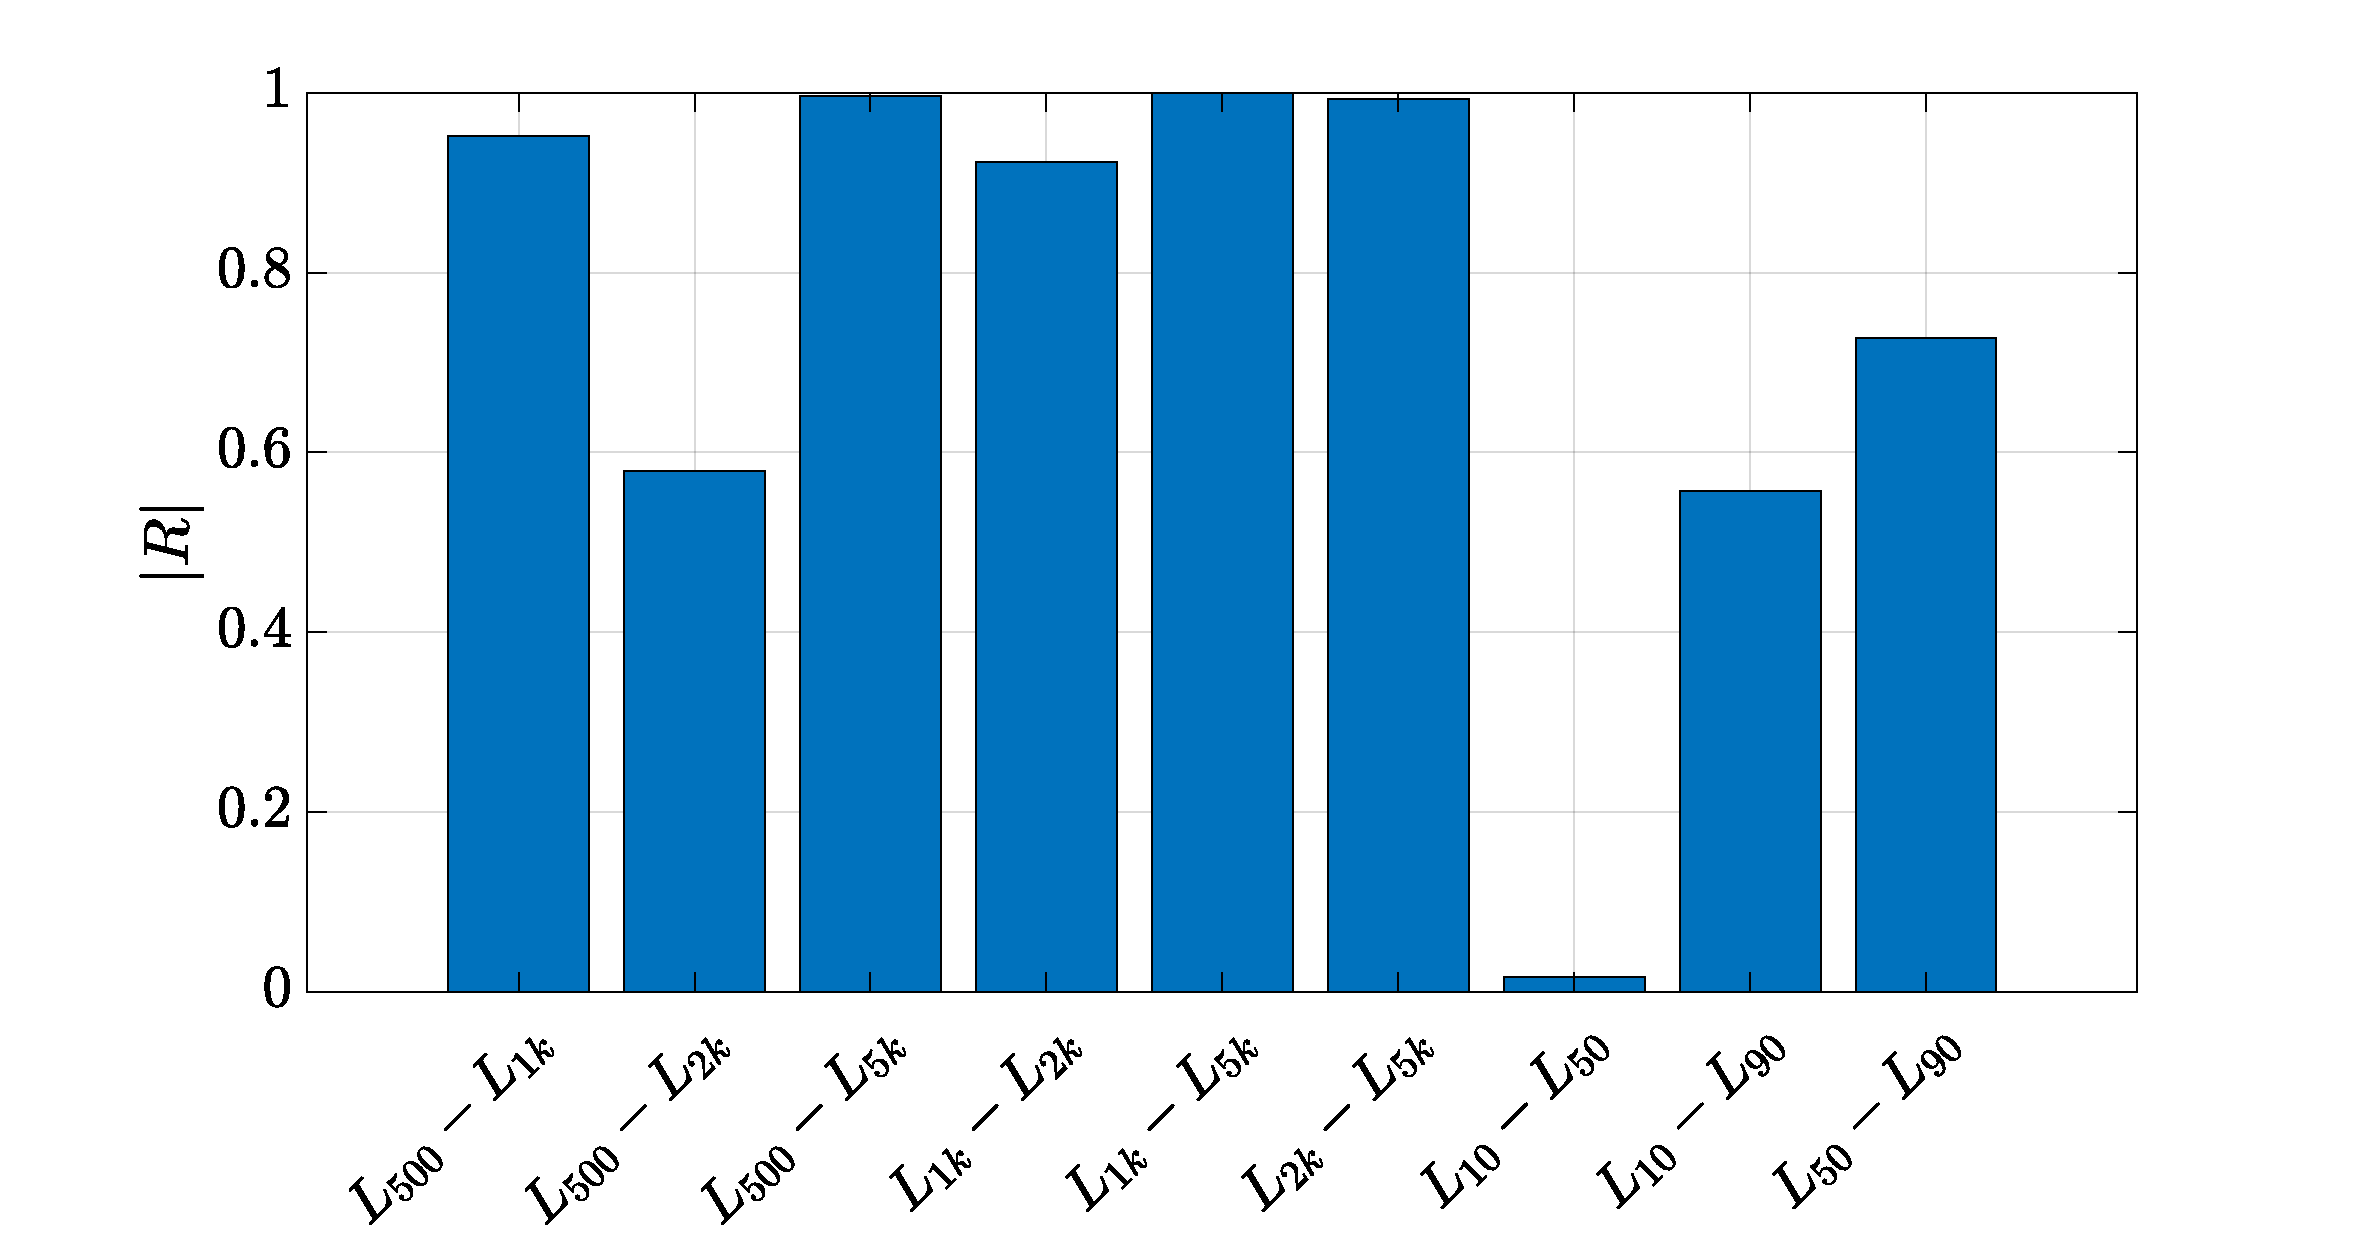
\includegraphics[width=0.9\linewidth]{./figures/resultats/Opt_correlation.pdf}
\caption{Corrélations entre l'évolution des seuils optimaux et des indicateurs $\Delta_{L_x-L_y}$.}
\label{fig:correlation}
\end{figure}

On obtient une forte corrélation pour les indicateurs $\Delta_{L_{1k}-L_{5k}}$, $\Delta_{L_{500}-L_{5k}}$ et $\Delta_{L_{2k}-L_{5k}}$. Avec une différence entre un niveau situé dans les basses (500 Hz) ou moyennes fréquences (1 kHz et 2 kHz) basses avec une niveau dans les plus hautes fréquences (5 kHz), on réussit à définir aux mieux les environnements sonores. Les ambiance \textit{Parc} et \textit{Rue calme} avec la présence d'oiseaux sont susceptibles de contenir plus de hautes fréquences alors que la source \textit{trafic} est moins présente. À l'inverse, pour les rues \textit{bruyante} et \textit{très bruyante}, celle-ci possèdent une plus grande proportion dans les basses fréquences. 
Les indicateurs basés sur la différence des niveaux fractiles et celui basé sur la différence entre le niveaux sonores des bandes de 500 Hz et de 2 kHz sont ceux obtenant les plus faibles corrélation. On observe que là où les autres indicateurs suit une évolution quasi linéaire, comme celle des seuils optimaux, ces 4 indicateurs ont des valeurs plus faibles pour l'ambiance \textit{calme}, ce qui ne permet pas d'obtenir une forte corrélation.

De ces indicateurs et des ces seuils optimaux, la NMF IS est de nouveaux appliqué sur le corpus \textit{SOUR} où la valeur du seuil $t_h$ n'est plus définie au préalable mais à partir de l'estimation d'un des indicateurs : pour chaque scène, un indicateur est calculé, puis, la valeur seuil $t_h$ est trouvée par interpolation (voir Figure \ref{fig:interpolation}). Toutefois, si l'indicateur $\Delta_L$ de la scène excède les valeurs limites déterminés aux ambiances \textit{parc} et \textit{rue très bruyante}, les seuils prennent les valeurs optimales de ces ambiance.  À partir de l'évolution de l'indicateur en fonction des valeurs seuil, on réalise une simple interpolation pour déterminer un seuil $t_h$ plus précis qui s'adapte ainsi à chaque scène sonore.


\begin{figure}[h]
\centering
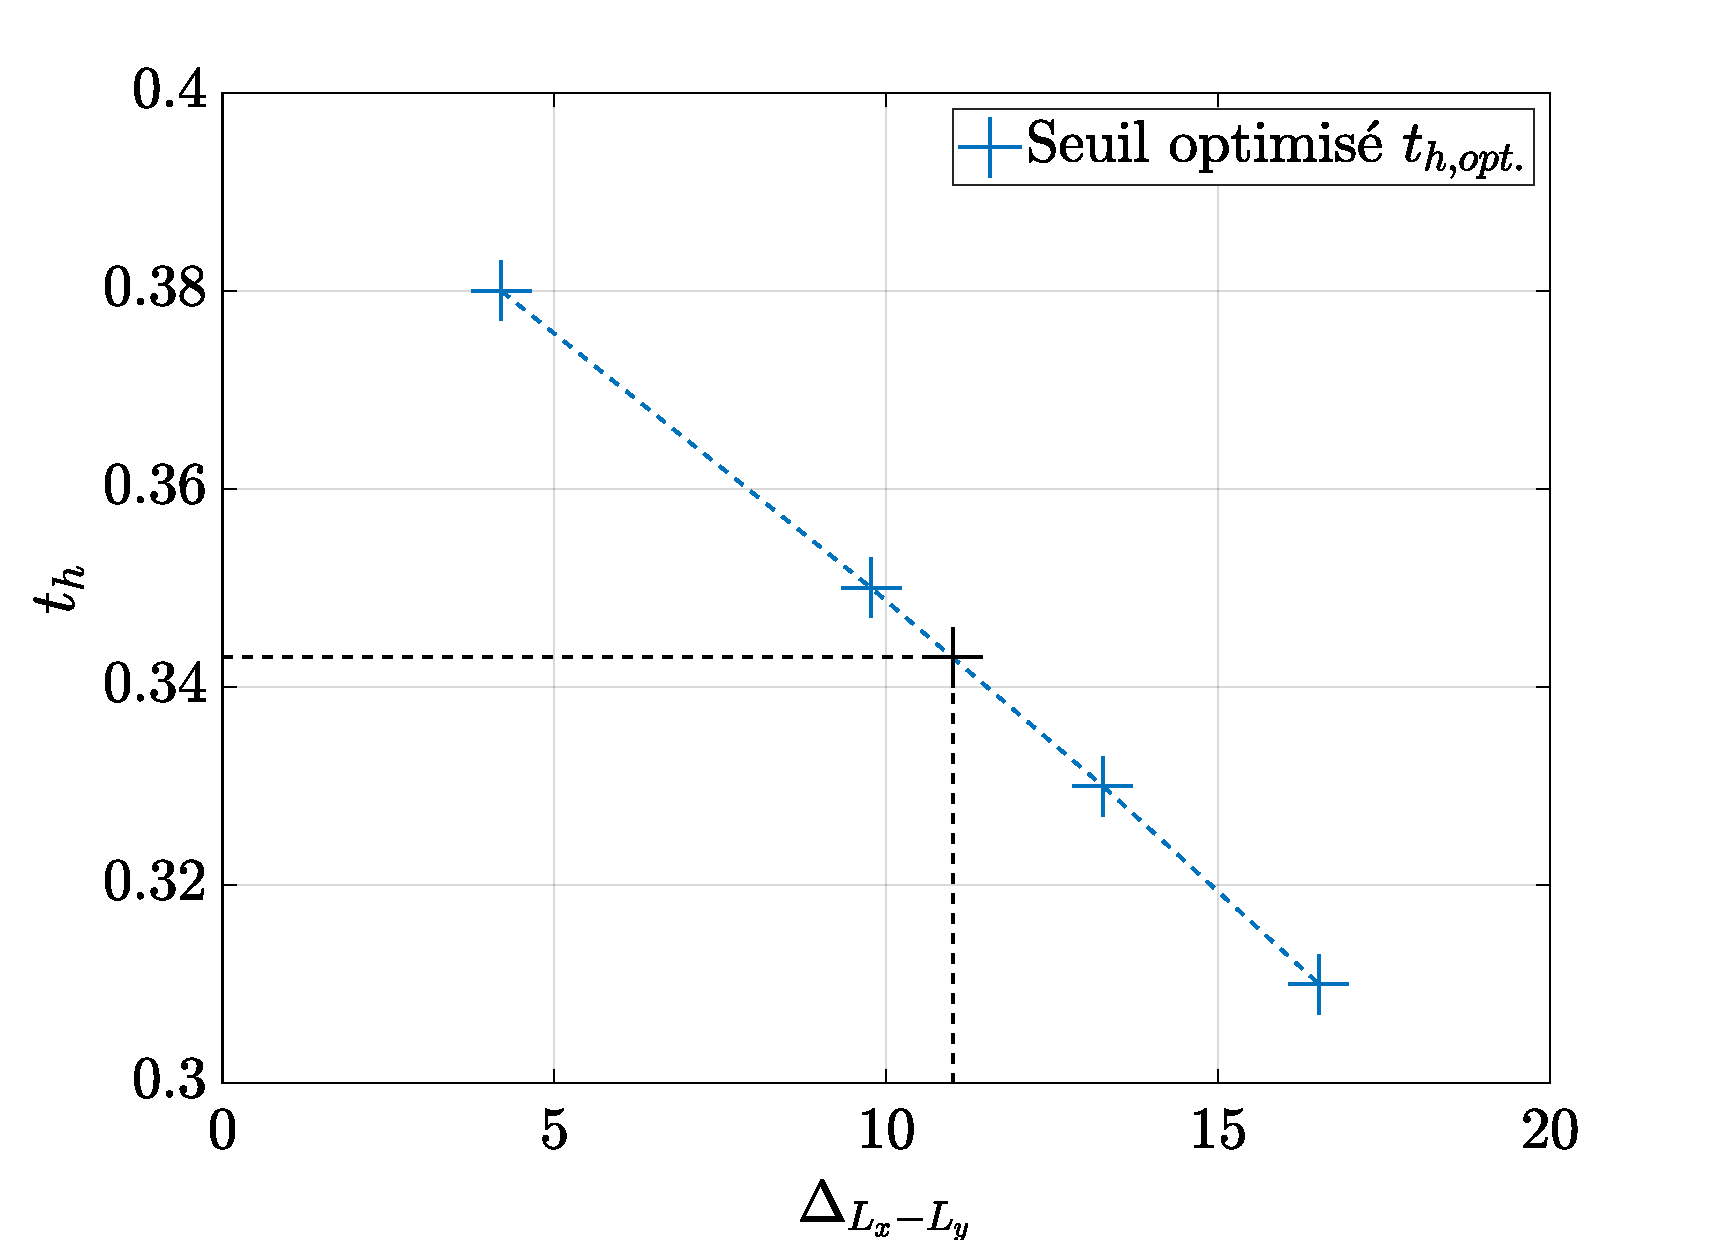
\includegraphics[width=.7\linewidth]{./figures/resultats/interpolationOpt.pdf}
\caption{Exemple d'interpolation réalisée pour une scène avec un indicateur $\Delta_{L_{1k}-L_{5k}}$ = 11 : $t_{h,interp}$ = 0,343.}
\label{fig:interpolation}
\end{figure}

\begin{table}[h]
\centering
\caption{Influence de l'indicateur d'optimisation dans l'estimation de l'erreur $MAE_{60}$.}
\label{tab:result_opt}
\begin{tabular}{L{3cm}C{2.5cm}}
\toprule
 & $MAE_g$    \\
 \midrule
seuil fixe & 1,16 ($\pm$ 0,86)  \\
\rowcolor[HTML]{C0C0C0}
seuil optimisé $t_{h,opt}$ & 1,12 ($\pm$ 0,83) \\
\midrule
\textcolor{red}{$\mathbf{\Delta_{L_{1k}-L_{5k}}}$} & \textbf{\textcolor{red}{1,08 ($\pm$ 0,87)}}\\
\rowcolor[HTML]{C0C0C0}
$\mathbf{\Delta_{L_{2k}-L_{5k}}}$& \textbf{1,09 ($\pm$ 0,86)}\\
$\Delta_{L_{500}-L_{5k}}$ & 1,12 ($\pm$ 0,90)\\
\rowcolor[HTML]{C0C0C0}
$\Delta_{L_{1k}-L_{2k}}$ & 1,12 ($\pm$ 0,93)\\
$\Delta_{L_{500}-L_{1k}}$ & 1,12 ($\pm$ 0,95)\\
\rowcolor[HTML]{C0C0C0}
$\Delta_{L_{50}-L_{90}}$ & 1,18 ($\pm$ 0,92)\\
$\Delta_{L_{10}-L_{90}}$ & 1,29 ($\pm$ 1,09)\\
$\Delta_{L_{10}-L_{50}}$ & 1,36 ($\pm$ 1,05)\\
\rowcolor[HTML]{C0C0C0}
$\Delta_{L_{500}-L_{2k}}$ & 1,37 ($\pm$ 1,16)\\
\bottomrule
\end{tabular}
\end{table}

Les erreurs $MAE_g$ obtenues sur le corpus sont résumées dans le Tableau \ref{tab:result_opt}.
L'erreur $MAE_g$ par interpolation est plus faible que celle basé sur le seuil fixe et sur les seuils optimisés. Les deux indicateurs permettant d'obtenir les plus faibles erreurs sont basés sur les méthodes ayant la plus forte corrélation $R$ : $\Delta_{L_{1k}-L_{5k}}$ et $\Delta_{L_{2k}-L_{5k}}$.
La fonction d'interpolation pour $\Delta_{L_{1k}-L_{5k}}$ est alors sur l'intervalle $\Delta_{L_{1k}-L_{5k}} \in\left[1,22;~ 15,84 \right]$: 

\begin{equation}
t_{h,interp.} = 4,70\times 10^{-3} \times \Delta_{L_{1k}-L_{5k}} +0,37.
\end{equation}

La Figure \ref{fig:erreurInterp} représente les erreurs par ambiances sonores pour la NMF IS basées sur un seuil fixe $t_h$, les seuils optimisés $t_{h,opt.}$ et sur les seuils interpolés $t_{h,interp.}$.

\begin{figure}[h]
\centering
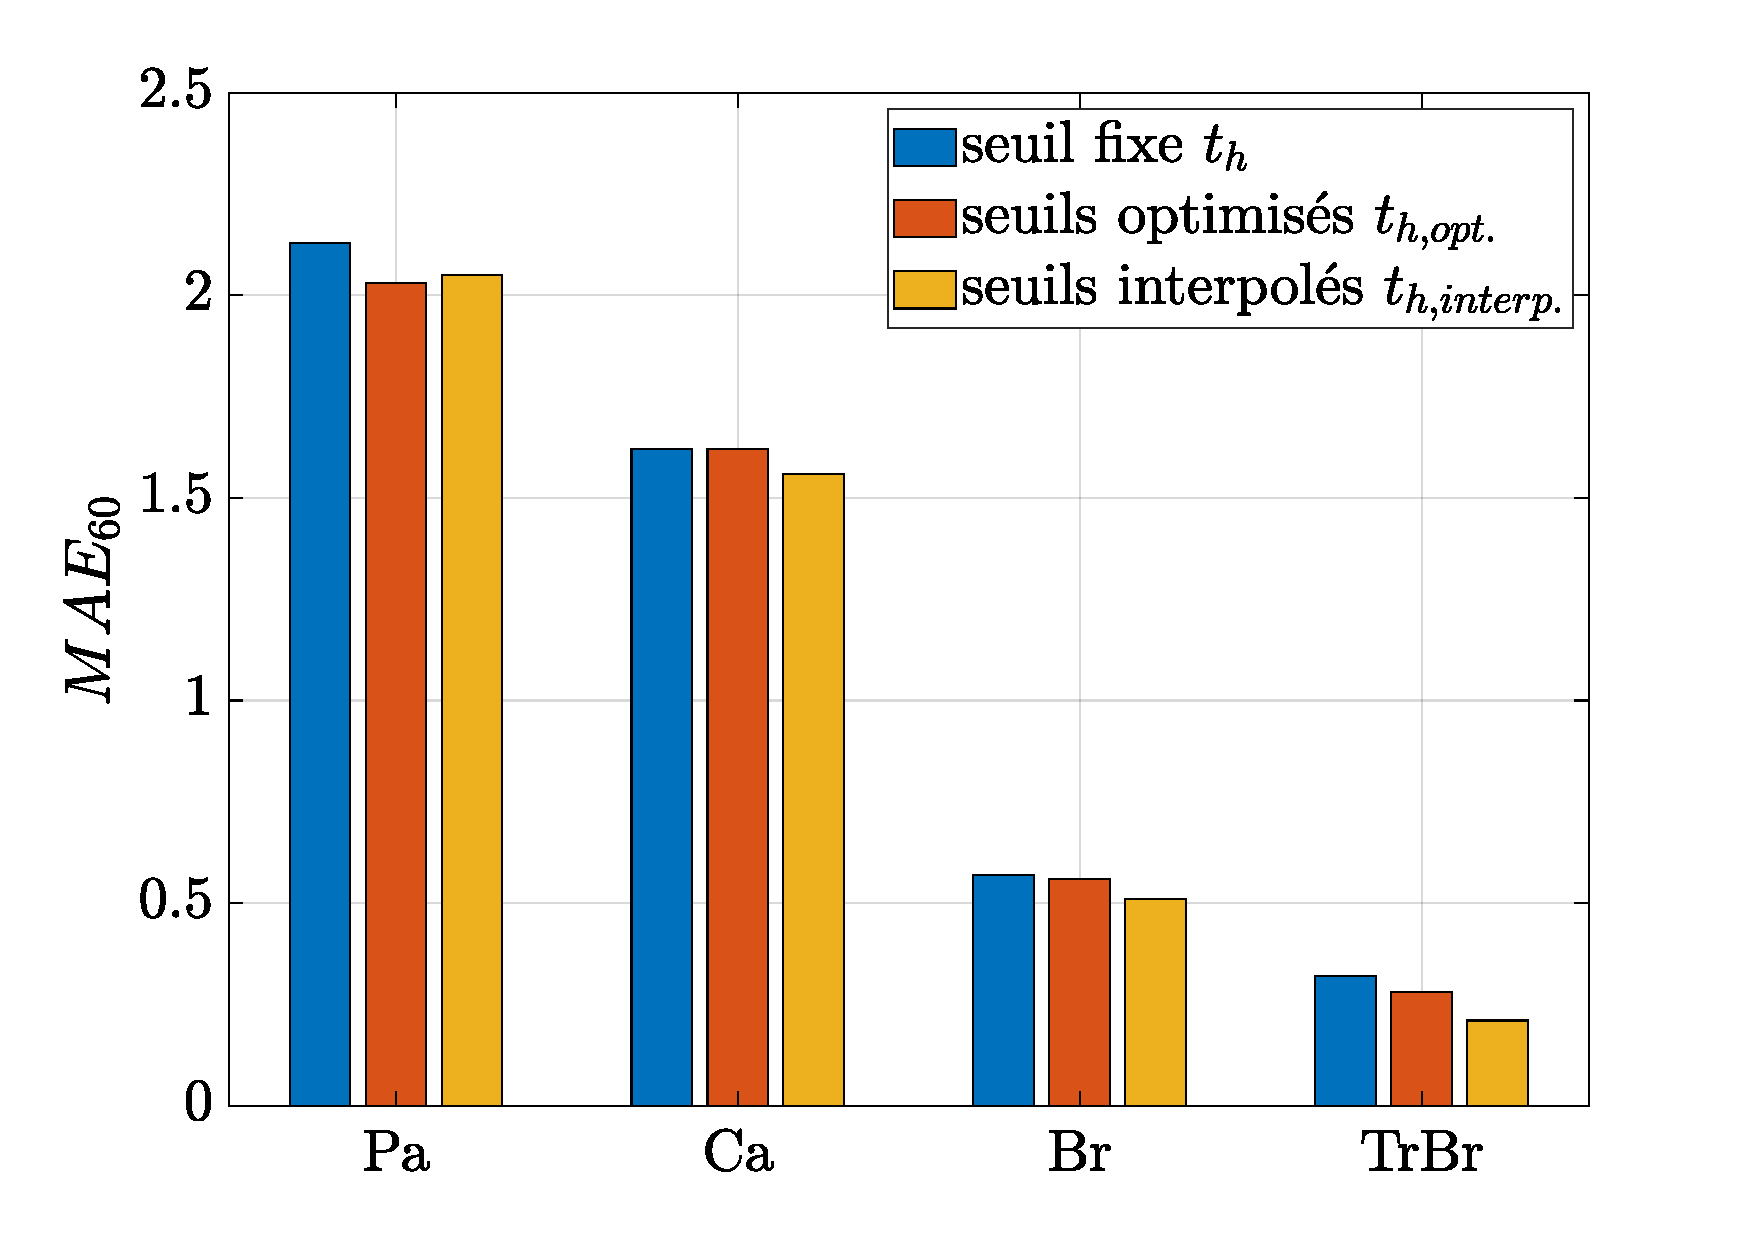
\includegraphics[width=.7\linewidth]{./figures/resultats/erreursSeuilOpt.pdf}
\caption{Influence de la méthode de seuillage (seul fixe $t_h$, optimisé $t_{h,opt.}$, interpolé $t_{h,intper.}$ à partir de l'indicateur $\Delta_{L_{1k}-L_{5k}}$) sur les erreurs $MAE_{60}$.}
\label{fig:erreurInterp}
\end{figure}

S'il y a bien une diminution de l'erreur, celle-ci reste relativement limitée. On constate que pour l'ambiance \textit{parc} est le seul cas où le seuil déduit de l'interpolation génère des erreurs supérieures aux deux autres approches. Cette particularité peut être mise en relation avec la sensibilité plus forte dans cette ambiance de l'erreur par rapport à la valeur du seuil (voir partie \ref{part:optimisationESU} et la Figure \ref{fig:maeExpandSeuil}). Dans les autres ambiances, la déduction du seuil par interpolation réduit les erreurs. 
Cette approche est une ouverture pour améliorer l'estimation du niveau sonore du trafic, elle reste à être validée sur des corpus plus grand et plus varié afin d'être plus juste. 
Mais cette proposition reste intéressante en vue d'adapter la méthode aux diverses environnements sonores : par un seuil variable déduit par des indicateurs sonore de la scène, il permet de mieux prendre en compte les évolutions sur la journée ou sur l'heure des ESU auprès du capteur.